\documentclass[
11pt, % The default document font size, options: 10pt, 11pt, 12pt
%codirector, % Uncomment to add a codirector to the title page
]{charter} 


% El títulos de la memoria, se usa en la carátula y se puede usar el cualquier lugar del documento con el comando \ttitle
\titulo{Título del proyecto} 

% Nombre del posgrado, se usa en la carátula y se puede usar el cualquier lugar del documento con el comando \degreename
%\posgrado{Carrera de Especialización en Sistemas Embebidos} 
%\posgrado{Carrera de Especialización en Internet de las Cosas} 
\posgrado{Carrera de Especialización en Inteligencia Artificial}
%\posgrado{Maestría en Sistemas Embebidos} 
%\posgrado{Maestría en Internet de las cosas}

% Tu nombre, se puede usar el cualquier lugar del documento con el comando \authorname
% IMPORTANTE: no omitir titulaciones ni tildación en los nombres, también se recomienda escribir los nombres completos (tal cual los tienen en su documento)
\autor{Título y Nombre del autor}

% El nombre del director y co-director, se puede usar el cualquier lugar del documento con el comando \supname y \cosupname y \pertesupname y \pertecosupname
\director{Título y Nombre del director}
\pertenenciaDirector{pertenencia} 
\codirector{} % para que aparezca en la portada se debe descomentar la opción codirector en los parámetros de documentclass
\pertenenciaCoDirector{FIUBA}

% Nombre del cliente, quien va a aprobar los resultados del proyecto, se puede usar con el comando \clientename y \empclientename
\cliente{Nombre del cliente}
\empresaCliente{Empresa del cliente}
 
\fechaINICIO{30 de abril de 2023}		%Fecha de inicio de la cursada de GdP \fechaInicioName
\fechaFINALPlan{18 de junio de 2023} 	%Fecha de final de cursada de GdP
\fechaFINALTrabajo{15 de mayo de 2024}	%Fecha de defensa pública del trabajo final


\begin{document}

\maketitle
\thispagestyle{empty}
\pagebreak


\thispagestyle{empty}
{\setlength{\parskip}{0pt}
\tableofcontents{}
}
\pagebreak


\section*{Registros de cambios}
\label{sec:registro}


\begin{table}[ht]
\label{tab:registro}
\centering
\begin{tabularx}{\linewidth}{@{}|c|X|c|@{}}
\hline
\rowcolor[HTML]{C0C0C0} 
Revisión & \multicolumn{1}{c|}{\cellcolor[HTML]{C0C0C0}Detalles de los cambios realizados} & Fecha      \\ \hline
0      & Creación del documento                                 &\fechaInicioName \\ \hline
%1      & Se completa hasta el punto 5 inclusive                & {día} de {mes} de 202X \\ \hline
%2      & Se completa hasta el punto 9 inclusive
%		  Se puede agregar algo más \newline
%		  En distintas líneas \newline
%		  Así                                                    & {día} de {mes} de 202X \\ \hline
%3      & Se completa hasta el punto 12 inclusive                & {día} de {mes} de 202X \\ \hline
%4      & Se completa el plan	                                 & {día} de {mes} de 202X \\ \hline

% Si hay más correcciones pasada la versión 4 también se deben especificar acá

\end{tabularx}
\end{table}

\pagebreak



\section*{Acta de constitución del proyecto}
\label{sec:acta}

\begin{flushright}
Buenos Aires, \fechaInicioName
\end{flushright}

\vspace{2cm}

Por medio de la presente se acuerda con el \authorname\hspace{1px} que su Trabajo Final de la \degreename\hspace{1px} se titulará ``\ttitle'' y consistirá en \textcolor{red}{la implementación de un prototipo de un sistema de control de temperatura de una caldera industrial}. El trabajo tendrá un presupuesto preliminar estimado de \textcolor{red}{600} horas y un costo estimado de \textcolor{red}{\$ XXX}, con fecha de inicio el \fechaInicioName\hspace{1px} y fecha de presentación pública el \fechaFinalName.

Se adjunta a esta acta la planificación inicial.

\vfill

% Esta parte se construye sola con la información que hayan cargado en el preámbulo del documento y no debe modificarla
\begin{table}[ht]
\centering
\begin{tabular}{ccc}
\begin{tabular}[c]{@{}c@{}}Dr. Ing. Ariel Lutenberg \\ Director posgrado FIUBA\end{tabular} & \hspace{2cm} & \begin{tabular}[c]{@{}c@{}}\clientename \\ \empclientename \end{tabular} \vspace{2.5cm} \\ 
\multicolumn{3}{c}{\begin{tabular}[c]{@{}c@{}} \supname \\ Director del Trabajo Final\end{tabular}} \vspace{2.5cm} \\
\end{tabular}
\end{table}




\section{1. Descripción técnica-conceptual del proyecto a realizar}
\label{sec:descripcion}

\begin{consigna}{red} % ELIMINAR \begin{consigna}{red} y \end{consigna}{red} en las secciones que vayan completando para cada entrega parcial.
El objetivo es que el lector, en una o dos páginas, exponga de qué se trata el proyecto y cuáles son sus desafíos, cuál es la motivación para realizarlo y su importancia.

Se debe introducir el contexto del proyecto, el estado del arte en la temática, describir la propuesta de valor, cuál es el problema que atiende y cuál es la solución que se propone. Se debe dar una descripción funcional de la solución que incluya un diagrama en bloques.

Puede ser útil incluir en esta sección la respuesta a alguna de estas preguntas:

\begin{itemize}
	\item ¿Cuál es el contexto del proyecto, es un emprendimiento personal, un proyecto para una empresa, es parte del programa de vinculación con empresas del posgrado?
	\item ¿Existen o aplican condiciones especiales al proyecto, financiamiento de algún programa público o privado, acuerdos de confidencialidad, acuerdos sobre la propiedad intelectual de los entregables u otros?
	\item ¿Cómo se compara la solución propuesta con el estado del arte en el campo de aplicación? ¿En qué aspectos destaca?
	\item ¿Ayuda a la explicación si se incluye un lienzo Canvas del Modelo de Negocio?
	\item ¿En qué estado del ciclo de vida está la solución que se propone?
	\item ¿Cuáles son las características del cliente (el adoptante de los entregables del proyecto) qué valora, qué necesita?
	\item ¿Por dónde pasa la innovación?
\end{itemize}

La descripción técnica-conceptual \textbf{debe incluir al menos un diagrama en bloques del sistema} y descripción funcional de la solución propuesta.

Las figuras se deben mencionar en el texto ANTES de que aparezcan con una frase como la siguiente: ``En la figura \ref{fig:diagBloques} se presenta el diagrama en bloques del sistema. Se observa que...''.  La regla es que las figuras nunca pueden ir antes de ser mencionadas en el texto, porque sino el lector no entiende por qué de pronto aparece una figura.

\begin{figure}[htpb]
\centering 
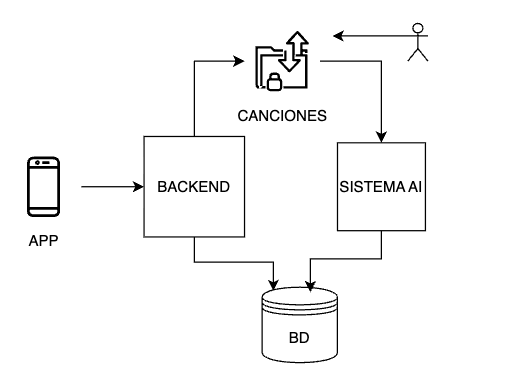
\includegraphics[width=.65\textwidth]{./Figuras/diagBloques.png}
\caption{Diagrama en bloques del sistema.}
\label{fig:diagBloques}
\end{figure}

\vspace{25px}

El tamaño del texto en TODAS las figuras debe ser adecuado \textbf{para que NO pase lo que ocurre en la figura \ref{fig:diagBloques}}, donde el lector debe esforzarse para poder leer el texto. 

Los colores usados en el diagrama deben ser adecuados, tal que ayuden a comprender mejor el diagrama. Se recomienda evitar colores primarios (como rojo, verde o cyan) y usar la gama de colores pastel.

\end{consigna} % ELIMINAR \begin{consigna}{red} y \end{consigna}{red} en las secciones que vayan completando para cada entrega parcial.

\section{2. Identificación y análisis de los interesados}
\label{sec:interesados}

\begin{consigna}{red} % ELIMINAR \begin{consigna}{red} y \end{consigna}{red} en las secciones que vayan completando para cada entrega parcial.
\textbf{Nota importante:} borrar esto y todas las consignas en color rojo antes de entregar este documento). Esto se hace eliminando el par de comandos que forman el bloque consigna, \verb!\begin{consigna}{red}! y \verb!\end{consigna}{red}! del código. 
 
Es inusual que una misma persona esté en más de un rol, incluso en proyectos chicos. Si se considera que una persona cumple dos o más roles, entonces \textbf{solo dejarla en el rol más importante}. 

Por ejemplo, si una persona es Cliente pero también colabora u orienta, dejarla solo como Cliente. Si una persona es el Responsable, \textbf{no debe ser colocado también como miembro del equipo}.


\begin{table}[ht]
%\caption{Identificación de los interesados}
%\label{tab:interesados}
\begin{tabularx}{\linewidth}{@{}|l|X|X|l|@{}}
\hline
\rowcolor[HTML]{C0C0C0} 
Rol           & Nombre y Apellido & Organización 	& Puesto 	\\ \hline
Auspiciante   &                   &              	&        	\\ \hline
Cliente       & \clientename      &\empclientename	&        	\\ \hline
Impulsor      &                   &              	&        	\\ \hline
Responsable   & \authorname       & FIUBA        	& Alumno 	\\ \hline
Colaboradores &                   &              	&        	\\ \hline
Orientador    & \supname	      & \pertesupname 	& Director del Trabajo Final \\ \hline
Equipo        & miembro1 \newline 
				miembro2          &              	&        	\\ \hline
Opositores    &                   &              	&        	\\ \hline
Usuario final &                   &              	&        	\\ \hline
\end{tabularx}
\end{table}

El Director suele ser uno de los orientadores.

No dejar celdas vacías; si no hay nada que poner en una celda colocar un signo ``-''.

No dejar filas vacías; si no hay nada que poner en una fila entonces eliminarla.

Es deseable listar a continuación las principales características de cada interesado.
 
Por ejemplo:
\begin{itemize}
	\item Orientador: la Dra. Ing. María Gómez es experta en la temática y va a ayudar con la definición de los requerimientos y el desarrollo del firmware del embebido.
	\item Auspiciante: es riguroso y exigente con la rendición de gastos. Tener mucho cuidado con esto.
	\item Equipo: Juan Perez, suele pedir licencia porque tiene un familiar con una enfermedad. Planificar considerando esto.
\end{itemize}

\end{consigna} % ELIMINAR \begin{consigna}{red} y \end{consigna}{red} en las secciones que vayan completando para cada entrega parcial.


\section{3. Propósito del proyecto}
\label{sec:proposito}

\begin{consigna}{red} % ELIMINAR \begin{consigna}{red} y \end{consigna}{red} en las secciones que vayan completando para cada entrega parcial.

¿Por qué se hace el proyecto? ¿Qué se quiere lograr? 

Se recomienda que sea solo un párrafo que continúe con la idea de la frase ``el propósito de este proyecto es...'' (omitir la frase, ya que está en el título de la sección).
\end{consigna}

\section{4. Alcance del proyecto}
\label{sec:alcance}

\begin{consigna}{red}
¿Qué se incluye y que no se incluye en este proyecto?

Se refiere al trabajo que se va a hacer para entregar el producto o resultado especificado. 

Explicitar todo lo quede comprendido dentro del alcance del proyecto. Por ejemplo:

El proyecto incluye:
\begin{itemize}
	\item Ítem 1.
	\item Ítem 2.
		\begin{itemize}
		\item Subítem 1.
		\item Subítem 2.
		\item ...
		\end{itemize}
	\item ...
	
\end{itemize}

Explicitar además todo lo que no quede incluido (``El presente proyecto no incluye...'')

\end{consigna} % ELIMINAR \begin{consigna}{red} y \end{consigna}{red} en las secciones que vayan completando para cada entrega parcial.


\section{5. Supuestos del proyecto}
\label{sec:supuestos}

\begin{consigna}{red} % ELIMINAR \begin{consigna}{red} y \end{consigna}{red} en las secciones que vayan completando para cada entrega parcial.
``Para el desarrollo del presente proyecto se supone que: ...''

\begin{itemize}
	\item Supuesto 1.
	\item Supuesto 2.
	\item ...
\end{itemize}

Por ejemplo, se podrían incluir supuestos respecto a disponibilidad de tiempo y recursos humanos y materiales, sobre la factibilidad técnica de distintos aspectos del proyecto, sobre otras cuestiones que sean necesarias para el éxito del proyecto como condiciones macroeconómicas o reglamentarias.

\end{consigna} % ELIMINAR \begin{consigna}{red} y \end{consigna}{red} en las secciones que vayan completando para cada entrega parcial.

\section{6. Product Backlog}
\label{sec:backlog}

El Product Backlog debe organizarse en cuatro \textbf{\textit{\'{e}picas}} fundamentales del proyecto. Cada \'{e}pica debe contener al menos dos historias de usuario que describan funcionalidades clave.

El Product Backlog debe permitir interpretar cómo será el proyecto y su funcionalidad. Se deben indicar claramente las prioridades entre las historias de usuario y si hay alguna opcional.

Las historias de usuario deben ser breves, claras y medibles, expresando el rol, la necesidad y el propósito de cada funcionalidad. También deben tener una prioridad definida para facilitar la planificación de los sprints.

Cada historia de usuario debe incluir una ponderación en \textit{Story Points}, un número entero que representa el tama\~no relativo de la historia. El criterio para calcular los Story Points debe indicarse explícitamente.

Las historias deben seguir el formato: ``\textit{Como [rol], quiero [tal cosa] para [tal otra cosa]}''.

Las \'{e}picas deben estructurarse de la siguiente forma:

\begin{itemize}
  \item \textbf{\'{E}pica 1}
    \begin{itemize}
      \item HU1
      \item HU2
    \end{itemize}
  \item \textbf{\'{E}pica 2}
    \begin{itemize}
      \item HU3
      \item HU4
    \end{itemize}
  \item \textbf{\'{E}pica 3}
    \begin{itemize}
      \item HU5
      \item HU6
    \end{itemize}
  \item \textbf{\'{E}pica 4}
    \begin{itemize}
      \item HU7
      \item HU8
    \end{itemize}
\end{itemize}

\textbf{Reglas para definir historias de usuario:}
\begin{itemize}
  \item Ser concisas y claras.
  \item Expresarlas en términos cuantificables y medibles.
  \item No dejar margen para interpretaciones ambiguas.
  \item Indicar claramente su prioridad y si son opcionales.
  \item Considerar regulaciones y normas vigentes.
\end{itemize}

\section{7. Criterios de aceptación de historias de usuario}
\label{sec:criteriosAceptacion}

Los criterios de aceptación deben establecerse para cada historia de usuario, asegurando que se cumplan las condiciones necesarias para que la funcionalidad sea validada correctamente.

Cada historia debe tener criterios medibles, específicos y verificables. Deben permitir validar que se cumple con las necesidades del usuario.

Se estructuran de forma análoga a las \'{e}picas del backlog:

\begin{itemize}
  \item \textbf{\'{E}pica 1}
    \begin{itemize}
      \item Criterios de aceptación HU1
      \item Criterios de aceptación HU2
    \end{itemize}
  \item \textbf{\'{E}pica 2}
    \begin{itemize}
      \item Criterios de aceptación HU3
      \item Criterios de aceptación HU4
    \end{itemize}
  \item \textbf{\'{E}pica 3}
    \begin{itemize}
      \item Criterios de aceptación HU5
      \item Criterios de aceptación HU6
    \end{itemize}
  \item \textbf{\'{E}pica 4}
    \begin{itemize}
      \item Criterios de aceptación HU7
      \item Criterios de aceptación HU8
    \end{itemize}
\end{itemize}

\textbf{Reglas para definir criterios de aceptación:}
\begin{itemize}
  \item Medibles y verificables.
  \item Especificar cuándo una historia se considera completada.
  \item Incluir condiciones específicas.
  \item No ambiguos.
  \item Probables de testear funcional o técnicamente.
  \item Mínimo 3 criterios por HU.
\end{itemize}

\section{8. Fases de CRISP-DM}

\begin{enumerate}
  \item \textbf{Comprensión del negocio:} objetivo, valor agregado de IA, métricas de éxito.
  \item \textbf{Comprensión de los datos:} tipo, origen, cantidad, calidad.
  \item \textbf{Preparación de los datos:} características clave, transformaciones necesarias.
  \item \textbf{Modelado:} tipo de problema, algoritmos posibles.
  \item \textbf{Evaluación del modelo:} métricas de rendimiento.
  \item \textbf{Despliegue del modelo (opcional):} tipo de despliegue y herramientas.
\end{enumerate}

\section{9. Desglose del trabajo en tareas}
\label{sec:wbs}

A partir de cada Historia de Usuario (HU) definida en la sección 6, descomponer el trabajo en tareas técnicas concretas, medibles y acotadas en el tiempo.

\begin{itemize}
\item Seleccionar entre 2 y 3 tareas por cada historia de usuario.
\item Cada tarea debe estar claramente formulada, ser técnica, accionable y con una estimación horaria entre 2 y 8 horas.
\item Evitar tareas genéricas (como ''desarrollar funcionalidad´´) o demasiado amplias.
\item Si una tarea supera las 8 horas, debe dividirse en subtareas.
\item Indicar la prioridad relativa de cada tarea (Alta, Media o Baja).
\end{itemize}

\begin{table}[htpb]
\centering
\begin{tabularx}{\linewidth}{@{}|X|X|c|c|@{}}
\hline
\rowcolor[HTML]{C0C0C0}
Historia de usuario & Tarea técnica & Estimación & Prioridad \\ \hline
HU1 & Tarea 1 HU1 & 6 h & Alta \\ \hline
HU1 & Tarea 2 HU1 & 8 h & Alta \\ \hline
HU2 & Tarea 1 HU2 & 5 h & Media \\ \hline
HU2 & Tarea 2 HU2 & 6 h & Alta \\ \hline
... & ... & ... & ... \\ \hline
\end{tabularx}
\end{table}

\textbf{Criterios para estimar tiempos:}
\begin{itemize}
  \item Considerar la complejidad técnica, el nivel de incertidumbre y la experiencia previa.
  \item Evitar subestimar el esfuerzo: estimar el tiempo realista que llevaría implementar, testear y documentar cada tarea.
  \item Basar la estimación en la experiencia propia o en referencias de tareas similares.
\end{itemize}

\textbf{Sobre la prioridad:}
\begin{itemize}
  \item Asignar una prioridad relativa (Alta, Media o Baja) según la relevancia funcional de la tarea y su impacto en los entregables.
  \item Priorizar tareas que estén vinculadas a criterios de aceptación de las HU o que sean necesarias para desbloquear otras.
  \item Incluir tareas opcionales solo si están bien justificadas.
\end{itemize}

\textbf{Recomendaciones generales:}
\begin{itemize}
  \item -Enfocarse en tareas que surgen directamente de las HU planteadas.
  \item No es necesario cubrir las 600 horas del proyecto en esta sección: el foco está en el desglose de funcionalidades clave.
  \item Este trabajo será la base para organizar algunos de los sprints y elaborar el cronograma del proyecto, por lo que debe ser claro y realista.
\end{itemize}

\section{10. Planificación de Sprints}

Organizar las tareas técnicas del proyecto en sprints de trabajo que permitan distribuir de forma equilibrada la carga horaria total, estimada en 600 horas.

\textbf{Consigna:}
\begin{itemize}
  \item Completar una tabla que relacione sprints con HU y tareas técnicas correspondientes.
  \item Incluir estimación en horas para cada tarea.
  \item Indicar responsable y porcentaje de avance estimado o completado.
  \item Contemplar también tareas de planificación, documentación, redacción de memoria y preparación de defensa.
\end{itemize}

\textbf{Conceptos clave:}
\begin{itemize}
  \item Una \'{e}pica es una unidad funcional amplia; una historia de usuario es una funcionalidad concreta; un sprint es una unidad de tiempo donde se ejecutan tareas.
  \item Las tareas son el nivel más desagregado: permiten estimar tiempos, asignar responsables y monitorear progreso.
\end{itemize}

\textbf{Duración sugerida:}
\begin{itemize}
  \item Para un proyecto de 600 h, se recomienda planificar entre 10 y 12 sprints de aproximadamente 2 semanas cada uno.
  \item Asignar entre 45 y 50 horas efectivas por sprint a tareas técnicas.
  \item Reservar 100 a 120 h para actividades no técnicas (planificación, escritura, reuniones, defensa).
\end{itemize}

\textbf{Importante:}
\begin{itemize}
  \item En proyectos individuales, el responsable suele ser el propio autor.
  \item Aun así, desagregar tareas facilita el seguimiento y mejora continua.
\end{itemize}

\textbf{Conversión opcional de Story Points a horas:}
\begin{itemize}
  \item 1 SP \(\approx\) 2 h como referencia flexible.
  \item Tener en cuenta aproximaciones tipo Fibonacci.
\end{itemize}

\begin{table}[htpb]
\centering
\caption{Formato sugerido}
\begin{tabularx}{\linewidth}{@{}|l|l|X|c|l|c|@{}}
\hline
\rowcolor[HTML]{C0C0C0}
Sprint & HU o fase & Tarea & Horas / SP & Responsable & \% Completado \\ \hline
Sprint 0 & Planificación & Definir alcance y cronograma & 10 h & Alumno & 100\% \\ \hline
Sprint 0 & Planificación & Reunión con tutor/cliente & 5 h & Alumno & 50\% \\ \hline
Sprint 0 & Planificación & Ajuste de entregables & 6 h & Alumno & 25\% \\ \hline
Sprint 1 & HU1 & Tarea 1 HU1 & 6 h / 3 SP & Alumno & 0\% \\ \hline
Sprint 1 & HU1 & Tarea 2 HU1 & 10 h / 5 SP & Alumno & 0\% \\ \hline
Sprint 2 & HU2 & Tarea 1 HU2 & 7 h / 5 SP & Alumno & 0\% \\ \hline
... & ... & ... & ... & ... & ... \\ \hline
Sprint 5 & Escritura & Redacción memoria & 50 h / 34 SP & Alumno & 0\% \\ \hline
Sprint 6 & Defensa & Preparación exposición & 20 h / 13 SP & Alumno & 0\% \\ \hline
\end{tabularx}
\end{table}

\textbf{Recomendaciones:}
\begin{itemize}
  \item Verificar que la carga horaria por sprint sea equilibrada.
  \item Usar sprints de 1 a 3 semanas, acordes al cronograma general.
  \item Actualizar el \% completado durante el seguimiento del proyecto.
  \item Considerar un sprint final exclusivo para pruebas, revisión y ajustes antes de la defensa.
\end{itemize}


\section{11. Diagrama de Gantt (sprints)}
\label{sec:gantt}

Visualizar en un diagrama de Gantt la planificación temporal del proyecto, tomando como base los sprints definidos en la sección anterior. Debe contemplar todas las horas del proyecto.

Consigna:

\begin{itemize}

\item Elaborar un diagrama de Gantt que muestre la secuencia temporal de los sprints.

\item Cada fila debe representar un sprint (con su número o nombre), y el eje horizontal debe indicar el tiempo (en semanas o fechas concretas).

\item Las tareas técnicas derivadas de HU deben diferenciarse visualmente (por ejemplo, con un color distinto) de las tareas no técnicas (planificación, redacción, defensa).

\item Incluir todas las tareas estimadas en cada sprint.
\end{itemize}

Recomendaciones para el Gantt:

\begin{itemize}

	\item Podés usar herramientas gratuitas como TeamGantt, ClickUp, GanttProject, [Google Sheets], [Trello + Planyway], entre otras.
	\item Ordená los sprints de forma cronológica, comenzando con Sprint 0 (planificación) y finalizando con el sprint de defensa.
	\item Asegurate de reflejar la duración realista de cada sprint según tu disponibilidad y el cronograma general del posgrado.
	\item Incluí hitos importantes: reuniones, entregas parciales, defensa.
\end{itemize}


Incluir una imagen legible del diagrama de Gantt. Si es muy ancho, presentar primero la tabla y luego el gráfico de barras.



\section{12. Normativa y cumplimiento de datos (gobernanza)}

En esta sección se debe analizar si los datos utilizados en el proyecto están sujetos a normativas de protección de datos y privacidad, y en qué condiciones se pueden emplear.

\textbf{Aspectos a considerar:}
\begin{itemize}
  \item Evaluar si los datos están regulados por normativas como GDPR, Ley 25.326 de Protección de Datos Personales en Argentina, HIPAA u otras según jurisdicción y temática.
  \item Determinar si el uso de los datos requiere consentimiento explícito de los usuarios involucrados.
  \item Indicar si existen restricciones legales, técnicas o contractuales sobre el uso, compartición o publicación de los datos.
  \item Aclarar si los datos provienen de fuentes licenciadas, de acceso público o bajo algún tipo de autorización especial.
  \item Analizar la viabilidad del proyecto desde el punto de vista legal y ético, considerando la gobernanza de los datos.
\end{itemize}

Este análisis es clave para garantizar el cumplimiento normativo y evitar conflictos legales durante el desarrollo y publicación del proyecto.


\section{13. Gestión de riesgos}
\label{sec:riesgos}

\begin{consigna}{red}
a) Identificación de los riesgos (al menos cinco) y estimación de sus consecuencias:
 
Riesgo 1: detallar el riesgo (riesgo es algo que si ocurre altera los planes previstos de forma negativa)
\begin{itemize}
	\item Severidad (S): mientras más severo, más alto es el número (usar números del 1 al 10).\\
	Justificar el motivo por el cual se asigna determinado número de severidad (S).
	\item Probabilidad de ocurrencia (O): mientras más probable, más alto es el número (usar del 1 al 10).\\
	Justificar el motivo por el cual se asigna determinado número de (O). 
\end{itemize}   

Riesgo 2:
\begin{itemize}
	\item Severidad (S): X.\\
	Justificación...
	\item Ocurrencia (O): Y.\\
	Justificación...
\end{itemize}

Riesgo 3:
\begin{itemize}
	\item Severidad (S):  X.\\
	Justificación...
	\item Ocurrencia (O): Y.\\
	Justificación...
\end{itemize}


b) Tabla de gestión de riesgos:      (El RPN se calcula como RPN=SxO)

\begin{table}[htpb]
\centering
\begin{tabularx}{\linewidth}{@{}|X|c|c|c|c|c|c|@{}}
\hline
\rowcolor[HTML]{C0C0C0} 
Riesgo & S & O & RPN & S* & O* & RPN* \\ \hline
       &   &   &     &    &    &      \\ \hline
       &   &   &     &    &    &      \\ \hline
       &   &   &     &    &    &      \\ \hline
       &   &   &     &    &    &      \\ \hline
       &   &   &     &    &    &      \\ \hline
\end{tabularx}%
\end{table}

Criterio adoptado: 

Se tomarán medidas de mitigación en los riesgos cuyos números de RPN sean mayores a...

Nota: los valores marcados con (*) en la tabla corresponden luego de haber aplicado la mitigación.

c) Plan de mitigación de los riesgos que originalmente excedían el RPN máximo establecido:
 
Riesgo 1: plan de mitigación (si por el RPN fuera necesario elaborar un plan de mitigación).
  Nueva asignación de S y O, con su respectiva justificación:
  \begin{itemize}
	\item Severidad (S*): mientras más severo, más alto es el número (usar números del 1 al 10).
          Justificar el motivo por el cual se asigna determinado número de severidad (S).
	\item Probabilidad de ocurrencia (O*): mientras más probable, más alto es el número (usar del 1 al 10).
          Justificar el motivo por el cual se asigna determinado número de (O).
	\end{itemize}

Riesgo 2: plan de mitigación (si por el RPN fuera necesario elaborar un plan de mitigación).
 
Riesgo 3: plan de mitigación (si por el RPN fuera necesario elaborar un plan de mitigación).

\end{consigna}

\section{14. Sprint Review}
\label{sec:sprint_review}

La revisión de sprint (\emph{Sprint Review}) es una práctica fundamental en metodologías ágiles. Consiste en revisar y evaluar lo que se ha completado al finalizar un sprint. En esta instancia, se presentan los avances y se verifica si las funcionalidades cumplen con los criterios de aceptación establecidos. También se identifican entregables parciales y se consideran ajustes si es necesario.

Aunque el proyecto aún se encuentre en etapa de planificación, esta sección permite proyectar cómo se evaluarán las funcionalidades más importantes del backlog. Esta mirada anticipada favorece la planificación enfocada en valor y permite reflexionar sobre posibles obstáculos.

\textbf{Objetivo:} anticipar cómo se evaluará el avance del proyecto a medida que se desarrollen las funcionalidades, utilizando como base al menos cuatro historias de usuario del \emph{Product Backlog}.


Seleccionar al menos 4 HU del Product Backlog. Para cada una, completar la siguiente tabla de revisión proyectada:

\textbf{Formato sugerido:}
\begin{table}[htpb]
\renewcommand{\arraystretch}{1.5}
\begin{tabular}{|>{\raggedright\arraybackslash}m{2.5cm}|
                >{\raggedright\arraybackslash}m{2.3cm}|
                >{\raggedright\arraybackslash}m{3cm}|
                >{\raggedright\arraybackslash}m{3cm}|
                >{\raggedright\arraybackslash}m{3cm}|}
\hline
\rowcolor[HTML]{CCCCCC}
\textbf{HU seleccionada} & \textbf{Tareas asociadas} & \textbf{Entregable esperado} & \textbf{¿Cómo sabrás que está cumplida?} & \textbf{Observaciones o riesgos} \\
\hline
                         & Tarea 1 &                             &                                           &                                     \\ \cline{2-2}
\multirow{-2}{=}{HU1}    & Tarea 2 & \multirow{-2}{=}{Módulo funcional} & \multirow{-2}{=}{Cumple criterios de aceptación definidos} & \multirow{-2}{=}{Falta validar con el tutor} \\
\hline
                         & Tarea 1 &                             &                                           &                                     \\ \cline{2-2}
\multirow{-2}{=}{HU3}    & Tarea 2 & \multirow{-2}{=}{Reporte generado} & \multirow{-2}{=}{Exportación disponible y clara} & \multirow{-2}{=}{Requiere datos reales} \\
\hline
                         & Tarea 1 &                             &                                           &                                     \\ \cline{2-2}
\multirow{-2}{=}{HU5}    & Tarea 2 & \multirow{-2}{=}{Panel de gestión} & \multirow{-2}{=}{Roles diferenciados operativos} & \multirow{-2}{=}{Riesgo en integración} \\
\hline
                         & Tarea 1 &                             &                                           &                                     \\ \cline{2-2}
\multirow{-2}{=}{HU7}    & Tarea 2 & \multirow{-2}{=}{Informe trimestral} & \multirow{-2}{=}{PDF con gráficos y evolución} & \multirow{-2}{=}{Puede faltar tiempo para ajustes} \\
\hline
\end{tabular}
\end{table}

\section{15. Sprint Retrospective}    
\label{sec:sprint_retro}

La retrospectiva de sprint es una práctica orientada a la mejora continua. Al finalizar un sprint, el equipo (o el alumno, si trabaja de forma individual) reflexiona sobre lo que funcionó bien, lo que puede mejorarse y qué acciones concretas pueden implementarse para trabajar mejor en el futuro.

Durante la cursada se propuso el uso de la \textbf{Estrella de la Retrospectiva}, que organiza la reflexión en torno a cinco ejes:

\begin{itemize}
\item  ¿Qué hacer más?
\item  ¿Qué hacer menos?
\item  ¿Qué mantener?
\item  ¿Qué empezar a hacer?
\item  ¿Qué dejar de hacer?
\end{itemize}

Aun en una etapa temprana, esta herramienta permite que el alumno planifique su forma de trabajar, identifique anticipadamente posibles dificultades y diseñe estrategias de organización personal.

\textbf{Objetivo:} reflexionar sobre las condiciones iniciales del proyecto, identificando fortalezas, posibles dificultades y estrategias de mejora, incluso antes del inicio del desarrollo.


Completar la siguiente tabla tomando como referencia los cinco ejes de la Estrella de la Retrospectiva (\emph{Starfish} o estrella de mar). Esta instancia te ayudará a definir buenas prácticas desde el inicio y prepararte para enfrentar el trabajo de forma organizada y flexible. Se deberá completar la tabla al menos para 3 sprints técnicos y 1 no técnico.

\textbf{Formato sugerido:}

\begin{table}[htpb]
\renewcommand{\arraystretch}{1.4}
\begin{tabular}{|>{\raggedright\arraybackslash}p{1.8cm}|
                >{\raggedright\arraybackslash}p{2.3cm}|
                >{\raggedright\arraybackslash}p{2.3cm}|
                >{\raggedright\arraybackslash}p{2.3cm}|
                >{\raggedright\arraybackslash}p{2.3cm}|
                >{\raggedright\arraybackslash}p{2.3cm}|}
\hline
\rowcolor[HTML]{CCCCCC} 
\textbf{Sprint tipo y N°} & \textbf{¿Qué hacer más?} & \textbf{¿Qué hacer menos?} & \textbf{¿Qué mantener?} & \textbf{¿Qué empezar a hacer?} & \textbf{¿Qué dejar de hacer?} \\
\hline
Sprint técnico - 1 & Validaciones continuas con el alumno & Cambios sin versión registrada & Pruebas con datos simulados & Documentar cambios propuestos & Ajustes sin análisis de impacto \\
\hline
Sprint técnico - 2 & Verificar configuraciones en múltiples escenarios & Modificar parámetros sin guardar historial & Perfiles reutilizables & Usar logs para configuración & Repetir pruebas manuales innecesarias \\
\hline
Sprint técnico - 8 & Comparar correlaciones con casos previos & Cambiar parámetros sin justificar & Revisión cruzada de métricas & Anotar configuraciones usadas & Trabajar sin respaldo de datos \\
\hline
Sprint no técnico - 12 (por ej.: ``Defensa'') & Ensayos orales con feedback & Cambiar contenidos en la memoria & Material visual claro & Dividir la presentación por bloques & Agregar gráficos difíciles de explicar \\
\hline
\end{tabular}
\end{table}




\end{document}